\section{Idealized Stenosis Case Study}
\label{sec:case-study}
\label{sec:idealized-stenosis-case-study}

This chapter applies the review framework to a controlled stenosis computation.
The example uses a smooth idealized vessel geometry and a one-dimensional
area--flow model with specified wall, profile, rheology, boundary, and numerical
choices. Its purpose is to show how a reduced-model comparison should be read
once the model state, discrete operator, observation map, and discrepancy metric
are fixed.

The evidence has three parts. A manufactured-solution test checks the forced
finite-volume operator against a known smooth solution. A geometry-rest test
evaluates whether the MUSCL/Rusanov scheme used here preserves the quiescent
stenotic equilibrium admitted by the continuous source-balanced model. A
final-time resolved-velocity comparison maps both the one-dimensional solution
and available three-dimensional velocity data to common section-mean
observables. These checks support a bounded diagnostic comparison, not a
clinical prediction or a full transient FSI validation study.

Figure~\ref{fig:stenosis-fem-fvm-meshes} orients the case study only: it
previews the stationary-Stokes finite-element sampling geometry and the
one-dimensional finite-volume grid before the model specification and evidence
categories are stated.

\begin{figure}[!htb]
    \centering
    \captionsetup{aboveskip=2pt,belowskip=2pt}
    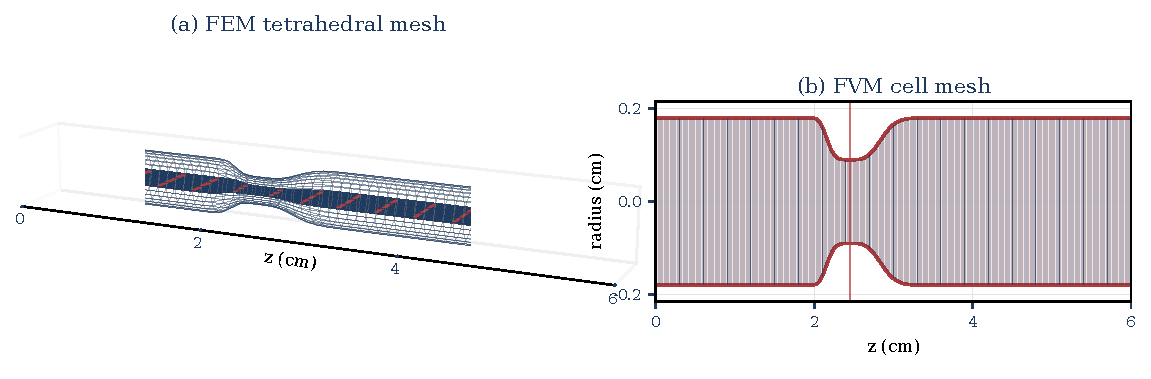
\includegraphics[width=\textwidth]{report/assets/rendered/stenosis-fem-fvm-meshes.pdf}
    \caption{Finite-element and finite-volume discretization views of the same
    $C^\infty$ reference stenosis geometry defined in
    Definition~\ref{def:1d-stenosis-reference-geometry}. Panel (a) shows a
    meridional projection of the stationary-Stokes tetrahedral mesh
    $\mathcal T_h$ against the wall curves $r=\pm R_0(z)$; the inset sketches a
    section $S_j=\Omega_{3D}\cap\{z=z_j\}$, the centroid-fan cut triangles
    $\mathcal Q_j$, and the three barycentric quadrature points used by the
    specified cross-section quadrature operator. Panel (b) shows the 1D
    finite-volume partition $I_i=[z_{i-1/2},z_{i+1/2}]$ with centers
    $z_i=(i-\frac12)\Delta z$, sampled along $R_0(z)$.}
    \label{fig:stenosis-fem-fvm-meshes}
\end{figure}

\subsection{Case-Study Role and Model Contract}
\label{sec:methodology}

This section applies the review framework to one controlled stenosis example.
It identifies the model tier, native variables, closure choices, boundary
approximation, principal numerical method, observation operator, and evidence
contract before any result is interpreted. Dense operator formulas, secondary
solver surfaces, and reproducibility commands remain in the appendices unless
they are needed to understand a main-body claim.

\begin{center}
\fbox{\begin{minipage}{0.90\linewidth}
\small
\textbf{Solver-coordinate convention.} In the comparison record, the stored
solver state \texttt{A} is $a=R^2$, not physical circular area. The physical
map is Definition~\ref{def:physical-to-solver-map}:
$A_{\mathrm{phys}}=\pi a$, $Q_{\mathrm{phys}}=\pi q$, and
$\bar u=q/a=Q_{\mathrm{phys}}/A_{\mathrm{phys}}$.
\end{minipage}}
\end{center}

\begin{table}[!htb]
    \centering
    \scriptsize
    \caption{Case-study contract for the retained 23\% and 40\%
    stenosis-severity numerical evidence.
    The table states the minimum computational and interpretive commitments
    needed before the result tables are read. It is a reading contract, not an
    additional numerical result.}
    \label{tab:t1-case-study-contract}
    \begin{tabularx}{\textwidth}{@{}
        >{\raggedright\arraybackslash}p{0.20\textwidth}
        >{\raggedright\arraybackslash}p{0.39\textwidth}
        >{\raggedright\arraybackslash}X@{}}
        \toprule
        \textbf{Contract item}
            & \textbf{Main-body statement}
            & \textbf{Interpretation boundary} \\
        \midrule
        Case-study purpose
            & A controlled idealized stenosis example applies the review
            framework to a selected 1D area--flow model and two resolved
            velocity fields.
            & The chapter illustrates verification, reproducibility, and
            diagnostic cross-model velocity comparison; it is not a
            pressure-ratio study or patient-specific prediction. \\
        Resolved datasets and final-time match
            & The retained resolved datasets are the 23\% stenosis case from
            local dataset 77 and the 40\% stenosis case from local dataset 60.
            Both are compared at $T=0.9995$ s, with recorded 1D--3D final-time
            offsets of $5.47\times10^{-14}$ s.
            & The final timestamp is matched. Earlier transient-history
            matching is not carried by the retained record and would be needed
            for a stronger predictive comparison. \\
        Principal 1D computation
            & The main comparison uses the $R_{\max}$-normalized
            Canic-derived extended 1D member with Newtonian
            $\nu=0.04$ cm$^2$/s, parabolic profile closure, $N=400$ MUSCL
            finite-volume cells, Rusanov flux, and native SSPRK3 time
            integration.
            & Other finite-volume, DG, timestepper, and descriptor records are
            implementation-health or sensitivity context rather than the
            principal two-case comparison method. \\
        Observation operator
            & The 3D velocity field is reduced by the declared
            \texttt{CrossSectionQuadratureOperator}; the 1D state is observed as
            physical flow $Q_{1D}=\pi q$ and mean velocity
            $\bar u_{1D}=q/a$ on 200 axial sections. A second retained
            comparison applies the resolved displacement field before forming
            the same plane cuts.
            & The comparison is meaningful only for these common section
            observables. Radial-profile outputs are retained only as an audit
            record because their area-closure gate fails. \\
        Numerical admissibility gates
            & The main text reports manufactured-solution behavior,
            output-operator verification, geometry-rest drift, subcritical
            boundary diagnostics, CFL, positivity, and finite-volume
            bookkeeping.
            & These records support run admissibility and numerical
            interpretation. They do not by themselves identify a physical
            prediction target. \\
        Matching limits
            & The analytic reference profile is shared and the static cut-area
            check is reported for both reference and deformed coordinates. A
            quasi-static membrane-FSI comparator is also retained for the
            radial wall displacement solve.
            & Velocity differences cannot be attributed uniquely to a specific
            closure, wall, boundary, or geometry mechanism because the retained
            resolved record still lacks matched boundary histories and full
            transient wall history. \\
        Retained outputs
            & The retained numerical evidence is the MMS/rest-state record,
            cut-area check, axial flow behavior, flow/area bookkeeping,
            section-mean velocity discrepancy summary, coordinate-mode
            comparison, quasi-static membrane-FSI wall summary,
            production-grid sensitivity, and largest section discrepancies.
            & These are descriptive final-time discrepancy and sensitivity
            records for the declared two-case comparison. \\
        Excluded radial/profile outputs
            & Secondary radial-profile rows were regenerated for selected
            axial slices and audited.
            & The raw rows reproduce the generated radial summary, but the
            area-closure gate fails because the radial slices do not coincide
            with the retained section-target set. \\
        \bottomrule
    \end{tabularx}
\end{table}

\subsubsection{Model Contract and Native Variables}
\label{subsec:methodology-problem-definition}
\label{subsec:selected-1d-forward-model}
\label{subsec:cross-sectional-variables-governing-equations}
\label{subsubsec:cross-sectional-reduction-selected-1d-model}

The computational problem is a single idealized stenotic vessel represented by a
selected one-dimensional area--flow model. The model assumes a distinguished
axial direction and cross-sectionally averaged pressure and velocity, retaining
distributed pulse-wave and pressure--flow structure while discarding secondary
flow, separation, recirculation, and resolved wall traction. The reduction
follows standard compliant-artery and dimension-reduced modeling arguments
\cite[Sec.~2, pp.~253--257]{FormaggiaEtAl2003OneDimensionalBloodFlow}
\cite[Ch.~3, Secs.~3.2 and~3.6]{KopplHelmig2023DimensionReducedModeling}
\cite[Sec.~3, pp.~24--26]{ShiEtAl2011BloodFlowModelReview}.

\begin{assumption}[Straight single-vessel geometry]
    \label{ass:1d-straight-vessel-geometry}
    The selected 1D model assumes a vessel of length $L$ aligned with the
    $z$-axis and a circular cross-section with radius $R(z,t)$. For
    $0<z<L$, $S(z,t)$ is the interior cross-section used for averaging, not
    a boundary component of the open lumen.
\end{assumption}

\begin{definition}[Section-averaged fields and observed pressure]
    \label{def:section-averaged-1d-fields}
    The retained reduced kinematic variables and observed pressure
    representative are
    \begin{flalign*}
        \quad A_{\mathrm{phys}}(z,t) &\defined \int_{S(z,t)} 1 \, dS, &&
            \text{physical cross-sectional area}, \\
        \quad Q_{\mathrm{phys}}(z,t) &\defined \int_{S(z,t)} u_z \, dS, &&
            \text{physical volumetric flow rate}, \\
        \quad \bar u(z,t) &\defined
            \frac{Q_{\mathrm{phys}}(z,t)}{A_{\mathrm{phys}}(z,t)}, &&
            \text{mean axial velocity}, \\
        \quad \bar p_{3D,\mathrm g}(z,t) &\defined
            \frac{1}{A_{\mathrm{phys}}(z,t)}
            \int_{S(z,t)} p_{3D,\mathrm g} \, dS, &&
            \text{observed 3D cross-sectional mean gauge pressure}.
    \end{flalign*}
    Here $p_{3D,\mathrm g}$ is continuum pressure in the wall-law gauge frame.
    The observed representative $\bar p_{3D,\mathrm g}$ is distinct from the
    reduced wall-law pressure variable introduced below.
\end{definition}

\begin{definition}[Physical-to-solver map for the implemented 1D state]
    \label{def:physical-to-solver-map}
    The continuum 1D model uses physical area $A_{\mathrm{phys}}$ and
    physical flow $Q_{\mathrm{phys}}$. The implemented radius-squared solver
    instead stores
    \begin{flalign*}
        \quad
        a=R^2,\qquad q=\frac{Q_{\mathrm{phys}}}{\pi}.
        &&
    \end{flalign*}
    Thus
    \begin{flalign*}
        \quad
        A_{\mathrm{phys}}=\pi a,\qquad
        Q_{\mathrm{phys}}=\pi q,\qquad
        \bar u=\frac{Q_{\mathrm{phys}}}{A_{\mathrm{phys}}}=\frac{q}{a}.
        &&
    \end{flalign*}
    With $K=Eh/(1-\sigma^2)$ and the Canic conservative-form convention
    $R_0^*=R_{\max}$, the selected evolution wall law gives the solver elastic
    flux contribution recorded in Appendix~\ref{app:num-current-solver-operator}:
    \begin{flalign*}
        \quad
        \Psi_h(a)=\frac{K}{3\rho R_{\max}^2}a^{3/2},
        \qquad
        \pd_a\Psi_h(a)=\frac{K}{2\rho R_{\max}^2}\sqrt a.
        &&
    \end{flalign*}
    This map is the convention used by the
    Section~\ref{sec:resolved-3d-comparison} velocity and flow comparisons.
\end{definition}

\subsubsection{Closure Choices: Geometry and Wall Law}
\label{subsec:stenosis-geometry-implemented-coordinates}
\label{subsec:selected-wall-law-closure-model}

\begin{definition}[Stenosis reference geometry]
    \label{def:1d-stenosis-reference-geometry}
    A stenosis is encoded through the reference radius or reference area. Let
    $R_{\mathrm{base}}(z)$ be the nominal healthy radius and $s(z)\in[0,1)$
    a fractional radius-reduction profile. Then
    \begin{flalign*}
        \quad
        R_0(z) &= R_{\mathrm{base}}(z)\big(1-s(z)\big),
        &
        A_0(z) &= \pi R_0(z)^2.
        \numberthis\label{eq:1d-stenosis-area} &&
    \end{flalign*}
    The baseline idealized stenotic-vessel profile is the smooth asymmetric
    kernel
    \begin{flalign*}
        \quad
        g(z) &= z-z_s+\kappa
        \exp\left(-\frac{(z-z_a)^2}{2\sigma_a^2}\right),
        &
        \psi(z) &= \exp\left(-\lambda g(z)^4\right),
        \numberthis\label{eq:1d-stenosis-kernel} && \\
        \quad
        s(z) &= s_{\max}\psi(z), \qquad 0\leq s_{\max}<1.
        \numberthis\label{eq:1d-stenosis-profile} &&
    \end{flalign*}
    In the default centimeter-scale simulation record, $z_a=2.5\,\mathrm{cm}$,
    $z_s=3.4\,\mathrm{cm}$, $\sigma_a=1\,\mathrm{cm}$,
    $\kappa=0.95\,\mathrm{cm}$, and
    $\lambda=50\,\mathrm{cm}^{-4}$.
    This geometry is the baseline idealized simulation geometry for the worked
    example.
\end{definition}

\begin{remark}[Stenosis-profile and variable-radius boundary]
    \label{rmk:1d-stenosis-profile-scope}
    The profile in Eq.~\ref{eq:1d-stenosis-profile} is $C^\infty$ and
    rapidly localized rather than compactly supported. This smooth idealized
    geometry is the baseline for the reduced simulations in this report and is
    also useful for fixed-wall 3D studies: the same analytic radius profile
    supplies controlled derivatives, wall normals, severity variation, and
    repeatable mesh-refinement families without introducing segmentation noise.
    Canic et al.\ show that standard 1D variable-geometry models may miss
    stenotic pressure and velocity trends unless additional variable-radius
    terms are included \cite[Abstract; Secs.~1--2]{CanicEtAl2024Extended1DStenosis}.
    Those corrections are included by the \texttt{canic-extended-1d}
    forward-model descriptor; the \texttt{classical-1d-no-slip} descriptor is
    the parabolic-profile baseline that retains the same selected wall law but
    omits the Canic variable-radius corrections.
\end{remark}

\begin{definition}[Classical parabolic-profile 1D baseline]
    \label{def:classical-no-slip-1d-baseline}
    The classical baseline used as a model-family member is a
    parabolic-profile reduced model. A no-slip wall trace is compatible with a
    parabolic profile for fully developed Newtonian flow in a straight circular
    tube, but no-slip alone does not imply that profile in an unsteady stenotic
    vessel. The parabolic profile is therefore an independent cross-sectional
    closure with $\alpha_{\mathcal P}=4/3$ and $g_{\mathcal P}=4$. In the
    implementation manifests this member is recorded under the descriptor
    \texttt{classical-1d-no-slip}; in the mathematical discussion it is
    the classical parabolic-profile baseline. It keeps the same reduced state
    variables and selected Canic-derived pressure--area wall law as the
    extended 1D framework, but omits the Canic effective-alpha variable-radius
    correction. The descriptor \texttt{canic-extended-1d} names the
    $R_{\max}$-normalized Canic-derived extended-model member.
\end{definition}

\begin{definition}[Selected Canic--Koiter pressure--area wall law]
    \label{def:1d-elastic-wall-law}
    The selected elastic wall closure is the Canic--Koiter thin-wall
    pressure--area law for the reduced wall-law gauge pressure
    $p_{\mathcal W,\mathrm g}$. In conventional area notation it may be written
    \begin{flalign*}
        \quad p_{\mathcal W,\mathrm g}(A,z,t)
        =
        p_{\mathrm{ext}}(z,t)
        + \frac{\beta(z)}{A_0(z)}
            \left(\sqrt{A(z,t)}-\sqrt{A_0(z)}\right).
        \numberthis\label{eq:1d-wall-law} &&
    \end{flalign*}
    Here $A_0(z)$ is the reference area, $p_{\mathrm{ext}}$ is the external
    pressure, and $\beta(z)$ is a wall-stiffness parameter. In the
    radius-squared coordinate $a=R^2$ used by the implemented finite-volume
    evolution, the selected continuous source-balanced member uses the Canic
    conservative-form reference radius $R_0^*=R_{\max}$:
    \begin{flalign*}
        \quad
        p_{1,\mathrm g}(a,z,t)
        =
        p_{\mathrm{ext}}(z,t)
        +
        \frac{K}{R_{\max}^2}
        \left(\sqrt a-R_0(z)\right),
        \qquad
        K=\frac{Eh}{1-\sigma^2}. &&
    \end{flalign*}
    With $A=\pi a$ and $A_0=\pi R_0^2$, the conventional law in
    Eq.~\ref{eq:1d-wall-law} reduces to this selected member only when
    \begin{flalign*}
        \quad
        \beta(z)=\sqrt{\pi}\,K\,\frac{R_0(z)^2}{R_{\max}^2}. &&
    \end{flalign*}
    Thus the implemented evolution uses a constant reference-radius
    denominator, not the local $R_0^{-2}$ denominator. In this report
    $R_{\max}$ is the healthy reference-radius parameter used by the solver;
    for the default stenosis profile it equals $\max_zR_0(z)$. The selected
    comparison runs use the cgs numerical-record values
    $\rho=1.055\,\mathrm{g}/\mathrm{cm}^3$,
    $E=5.02\times10^6\,\mathrm{dyn}/\mathrm{cm}^2$,
    $h=0.06\,\mathrm{cm}$, $\sigma=0.5$,
    $K=4.016\times10^5\,\mathrm{dyn}/\mathrm{cm}$,
    $R_{\max}=0.18\,\mathrm{cm}$, and
    $p_{\mathrm{ext}}\equiv0$.
    This is the wall law paired with the implemented elastic potential and
    wall/geometry source below. Legacy pressure-output helpers in the
    implementation still report a local-denominator pressure diagnostic through
    \path{pressure(result, params)}; benchmark pressure extrema and
    pressure-diagnostic bars refer to that diagnostic, not to the selected
    evolution wall law. The 1D model identifies $p_{\mathcal W,\mathrm g}$ with
    a cross-sectional pressure representative as a closure assumption and does
    not resolve radial pressure variation.
\end{definition}

\subsubsection{Reduced Balance Law and Rest-State Contract}
\label{subsec:conservative-form-source-terms}

The selected 1D model is an area--flow balance law closed by the profile,
rheology, wall, geometry, and boundary choices stated above. In review terms,
the important point is that the model retains only axial area and flow while
moving transverse velocity, wall response, friction, rheology, and
variable-radius effects into closures. Appendix~\ref{app:num-current-solver-operator}
gives the corresponding semi-discrete operator in solver coordinates, including
the $R_{\max}$-normalized wall potential, wall/geometry source, friction term,
effective-alpha correction, and locally frozen $p_2$ derivative. The main-body
case study uses that appendix as the implementation authority and records here
only the model contract needed to interpret the evidence.

The continuous selected member has a rest state that matters for the evidence
standard. Under constant external pressure and compatible zero-flow boundary
data, the reference geometry $a(z)=R_0(z)^2$ with $q(z)=0$ should remain at
rest in the continuous source-balanced model. This property is the target of
the geometry-rest verification test in Section~\ref{subsec:rest-state-drift}.

\begin{proposition}[Rest-state compatibility of the selected wall source]
    \label{prop:selected-rest-state-compatibility}
    Suppose $p_{\mathrm{ext}}$ is constant in the gauge convention and the
    boundary data are compatible with $q=0$. Then
    $a(z)=R_0(z)^2$ and $q(z)=0$ are an exact steady state of the selected
    continuous source-balanced evolution law.
\end{proposition}

\begin{proof}
    Using the operator definitions in Appendix~\ref{app:num-current-solver-operator},
    the mass equation gives $\pd_z q=0$. In the momentum equation, all terms
    proportional to $q$ vanish, so
    $S_{\mathrm{fric}}=S_{\alpha}=S_{p_2}=0$. At $a=R_0^2$,
    \begin{flalign*}
        \quad
        \pd_z\Psi_h(R_0^2)
        &=
        \pd_z\left(\frac{K}{3\rho R_{\max}^2}R_0^3\right)
        =
        \frac{K}{\rho R_{\max}^2}R_0^2R_0'
        =
        S_{\mathrm{wall}}(R_0^2,z). &&
    \end{flalign*}
    Thus the elastic flux derivative is exactly canceled by the wall/geometry
    source, and $\pd_t q=0$.
\end{proof}

Continuous compatibility does not imply discrete preservation: the current
MUSCL/Rusanov method exhibits the reported non-well-balanced geometry-rest
drift.

\subsubsection{Source-to-Implementation Differences}
\label{subsec:source-to-implementation-variant}

The selected implementation is a documented Canic-derived extended model, not
a literal reproduction of every source-paper parameter and normalization in
\cite{CanicEtAl2024Extended1DStenosis}. The report therefore uses the phrase
\emph{$R_{\max}$-normalized Canic-derived extended model} when source fidelity
matters. Table~\ref{tab:source-to-implementation-model} records the relevant
source-to-implementation choices. The diagnostic extended pressure correction is
\begin{flalign*}
    \quad
    p_{2,\mathrm g}(a,q,z,t)
    =
    g_{\mathcal P}\rho\nu_{\mathrm{eff}}^{\mathcal R}
    \frac{q}{a}\frac{R_0'(z)}{R_0(z)}. &&
\end{flalign*}
This $p_2$ term is a variable-radius viscous correction, not a replacement wall
law. In generalized-Newtonian descriptor runs, the implemented analytic $p_2$
derivative uses the local value of $\nu_{\mathrm{eff}}^{\mathcal R}$ and does
not differentiate that effective-viscosity factor; it is therefore a locally
frozen-viscosity computational closure for this term.

\begin{table}[!htb]
    \centering
    \scriptsize
    \caption{Source-to-implementation map for the selected 1D model.}
    \label{tab:source-to-implementation-model}
    \begin{tabularx}{\textwidth}{@{}
        >{\raggedright\arraybackslash}p{0.24\textwidth}
        >{\raggedright\arraybackslash}p{0.34\textwidth}
        >{\raggedright\arraybackslash}X@{}}
        \toprule
        \textbf{Feature} & \textbf{Canic et al. source form} & \textbf{Implemented report form} \\
        \midrule
        Pressure denominator
            & Elastic pressure written with a local $R_0(z)^{-2}$ denominator.
            & Evolution wall potential and source use the constant
            $R_{\max}^{-2}$ normalization specified in
            Appendix~\ref{app:num-current-solver-operator}. \\
        Profile parameters
            & Source simulations state $\gamma=9$ and $\alpha=1.1$.
            & Principal runs use the parabolic profile
            $\alpha_{\mathcal P}=4/3$, $g_{\mathcal P}=4$; power-profile runs
            are sensitivity/diagnostic records. \\
        Friction coefficient
            & Profile-dependent wall/friction closure in the reduced model.
            & Implemented through the declared velocity-profile shear factor
            and rheology descriptor. \\
        $p_2$ differentiation
            & Variable-radius pressure correction differentiated in the model.
            & Locally frozen-viscosity treatment for the $p_2$ derivative. \\
        External pressure
            & External pressure term may be included in the formulation.
            & $p_{\mathrm{ext}}\equiv0$ in the reported runs. \\
        Coordinates
            & Physical area and flow notation in the source paper.
            & Solver state is $(a,q)$ with
            $A_{\mathrm{phys}}=\pi a$, $Q_{\mathrm{phys}}=\pi q$. \\
        Boundary rule
            & Boundary conditions are model/problem dependent.
            & Fixed-area characteristic approximation applied with persisted
            subcritical-regime diagnostics. \\
        Discrete well balancing
            & Continuous rest equilibrium is a model-level property.
            & Rusanov/MUSCL is not exactly well balanced for spatially varying
            $R_0$; Section~\ref{sec:numerical-verification} reports
            zero-forcing rest-state drift. \\
        \bottomrule
    \end{tabularx}
\end{table}

\subsubsection{Boundary Approximation and Subcritical Condition}
\label{subsec:initial-boundary-conditions}

The comparison runs start from the geometry-rest state and then impose the
finite-volume boundary approximation stated below.

\begin{definition}[Single-vessel boundary data]
    \label{def:1d-single-vessel-boundary-data}
    Generic single-vessel models may prescribe inlet flow or velocity and an
    outlet pressure or terminal relation; these alternatives are model-family
    context rather than the reported boundary rule. The realized finite-volume
    run prescribes an inlet solver flow derived from a nominal reference-area
    mean velocity,
    \begin{flalign*}
        \quad
        q_{\mathrm{in}}&=R_0(0)^2\bar u_{\mathrm{in}}, &&
    \end{flalign*}
    solves the inlet ghost area from the approximate outgoing characteristic
    invariant, fixes the outlet ghost coordinate
    $a_{\mathrm{out}}=R_0(L)^2$, and obtains the outlet ghost flow from the
    corresponding approximate invariant. Hence the imposed inlet condition is
    a prescribed reference-area flow, not a fixed realized mean velocity
    $q_{\mathrm{in}}/a_{\mathrm{in}}$, and the outlet condition fixes the
    elastic reference pressure only for the selected wall component.
\end{definition}

\begin{definition}[Characteristic speeds for the reduced elastic subsystem]
    \label{def:1d-characteristic-speeds}
    Let $\lambda_\pm$ denote the two characteristic speeds of the
    positive-area elastic 1D subsystem obtained from the homogeneous
    $(A,Q)$ balance law. Their formula and assumptions are given in
    Appendix~\ref{app:num-elastic-potential-form}.
\end{definition}

\begin{assumption}[Subcritical boundary regime]
    \label{ass:1d-subcritical-boundary-regime}
    The baseline boundary treatment is used only in the subcritical regime
    $\lambda_-<0<\lambda_+$, where one characteristic enters through the inlet
    and one characteristic enters through the outlet.
\end{assumption}

Under this regime, a finite-volume scheme constrains the incoming information at
each boundary and leaves the outgoing state determined by the interior solve.
The finite-volume boundary treatment in
Appendix~\ref{app:num-boundary-state-realization} uses an $\alpha=1$,
fixed-area characteristic approximation as the boundary invariant for the
variable-$\alpha_{\mathrm{eff}}$ solver. It is therefore an implemented boundary
approximation, not an exact invariant derivation for the full variable-radius
balance law.

\subsubsection{Principal MUSCL/Rusanov/SSPRK3 Method}
\label{subsec:muscl-ssprk3-discretization}

Only the principal comparison method belongs in the main narrative. The reported
two-case severity comparison uses the finite-volume method specified in
Appendix~\ref{app:num-current-solver-operator}: the radius-squared state
$(a,q)$ is advanced on a one-dimensional grid with MUSCL reconstruction,
minmod-limited conservative states, Rusanov flux, source splitting for the
wall/geometry and variable-radius terms, and native SSPRK3 time integration.
The principal numerical comparison uses $N=400$ cells on $0\le z\le6$ cm, a
timestep cap of $10^{-5}$ s, and a CFL cap of 0.45. The optional
output-sensitivity record reruns the same comparison protocol at
$N=200,400,800$ cells and is interpreted only as a production-grid sensitivity
check. The boundary-state approximation is the fixed-area characteristic
contract recorded in
Appendix~\ref{app:num-boundary-state-realization}. Other finite-volume, modal-DG,
native time-stepper, and SciML/OrdinaryDiffEq surfaces are implementation-check
or sensitivity context summarized in Table~\ref{tab:implemented-discretization-surface};
they are not the principal two-case comparison method.

\subsubsection{Plane--Tetrahedron Observation Operator}
\label{subsec:cross-sectional-velocity-reconstruction}
\label{subsec:plane-tetrahedron-comparison-operator}

The 1D state directly supplies a section mean,
$\bar u_{1D}(z,t)=q(z,t)/a(z,t)$, and physical flow
$Q_{1D}(z,t)=\pi q(z,t)$. The implementation can also emit radial-profile
rows using the same cut triangles. Those rows are audited in this manuscript,
but no radial-profile figure or localization claim is retained because the
radial area-closure gate fails.

The resolved-data loader also accepts pressure and displacement XDMF/HDF5
companions for a velocity field. When the comparison is explicitly run in
deformed-coordinate mode, the observation operator applies the node-centered
displacement before forming the plane cuts. Both the reference-coordinate and
deformed-coordinate section comparisons are retained in
Section~\ref{subsec:deformed-coordinate-comparison}.

For a target plane $S_j=\Omega_{\mathrm{3D}}\cap\{z=z_j\}$, the default
\texttt{CrossSectionQuadratureOperator} intersects every tetrahedron with
$S_j$, linearly interpolates axial velocity on the cut edges, sorts the cut
polygon vertices in the plane, and triangulates the polygon by a centroid fan.
Let $\mathcal Q_j$ denote the resulting cut triangles. The reported 3D area,
flow, and mean velocity are
\begin{flalign*}
    \quad
    A_{3D,j}
    &=
    \sum_{\Delta\in\mathcal Q_j}|\Delta|,
    &
    Q_{3D,j}
    &=
    \sum_{\Delta\in\mathcal Q_j}|\Delta|\,\bar u_{z,\Delta},
    &
    \bar u_{3D,j}
    &=
    Q_{3D,j}/A_{3D,j}. &&
\end{flalign*}
For a cut triangle $\Delta$ whose vertices carry reconstructed axial
velocities $u_{z,1}$, $u_{z,2}$, and $u_{z,3}$,
\begin{flalign*}
    \quad
    \bar u_{z,\Delta}
    =
    \frac{u_{z,1}+u_{z,2}+u_{z,3}}{3}. &&
\end{flalign*}
The corresponding 1D quantities use physical flow, not the raw solver flow
coordinate:
\begin{flalign*}
    \quad
    Q_{1D,j}
    =
    \pi q(z_j,t),
    \qquad
    \bar u_{1D,j}
    =
    q(z_j,t)/a(z_j,t). &&
\end{flalign*}
Quarantined radial rows are not part of the retained comparison metrics.

\subsubsection{Comparison Design and Discrepancy Metrics}
\label{subsec:numerical-experiments-metrics-provenance}

The resolved-velocity comparison evaluates the selected 1D solution against two
available resolved 3D velocity comparison datasets at the matched final-time
sample $T=0.9995$ s. The retained cases are described by their 23\% and 40\%
stenosis severities, with local dataset identifiers recorded only for
provenance. The comparison is a diagnostic cross-model velocity comparison
under the declared observation operator.
The compact reading contract is stated at the start of this section.
Regeneration commands, local source identifiers, raw-input policy, and static
asset ownership are recorded in
Appendix~\ref{app:code-and-ai-use}.

Velocity and flow differences are reported as sample discrepancy measures over
valid section targets. With
$d_{u,j}=\bar u_{1D,j}-\bar u_{3D,j}$ and
$d_{Q,j}=Q_{1D,j}-Q_{3D,j}$, the retained section metrics are the signed mean
bias, mean absolute discrepancy, RMS discrepancy, maximum absolute discrepancy,
and relative RMS discrepancy,
\begin{flalign*}
    \quad
    \overline d_u
    &=
    \frac{1}{n}\sum_j d_{u,j},
    &
    D_{u,1}
    &=
    \frac{1}{n}\sum_j |d_{u,j}|,
    &
    D_{u,2}
    &=
    \left(\frac{1}{n}\sum_j d_{u,j}^2\right)^{1/2}, &&\\
    \quad
    D_{u,\infty}
    &=
    \max_j |d_{u,j}|,
    &
    D_{u,2}^{\mathrm{rel}}
    &=
    \frac{\left(\sum_j d_{u,j}^2\right)^{1/2}}
         {\left(\sum_j\bar u_{3D,j}^2\right)^{1/2}}, &&\\
    \quad
    \overline d_Q
    &=
    \frac{1}{n}\sum_j d_{Q,j},
    &
    D_{Q,1}
    &=
    \frac{1}{n}\sum_j |d_{Q,j}|,
    &
    D_{Q,2}
    &=
    \left(\frac{1}{n}\sum_j d_{Q,j}^2\right)^{1/2}. &&
\end{flalign*}


\FloatBarrier

\subsection{Verification Evidence and Rest-State Preservation}
\label{sec:numerical-verification}

The worked example uses the evidence standards from
Section~\ref{sec:numerical-methods} in three ways: manufactured-solution
verification checks the forced finite-volume operator, the geometry-rest test
checks preservation of the declared zero-flow equilibrium by the selected
comparison method, and admissibility diagnostics report the boundary, CFL,
positivity, and conservation regime of the accepted comparison runs. Secondary
checks for nonprincipal numerical surfaces remain in
Appendix~\ref{app:numerical-methods-details}.

\subsubsection{Evidence Hierarchy and Scope}
\label{subsec:verification-scope-convergence-stability}

The hierarchy is explicit. The strongest positive result is the
manufactured-solution test, because it compares the implemented forced operator
with a specified smooth exact solution and an independently assembled forcing
consistency check. The geometry-rest test then checks the named stationary
family used to initialize the comparison runs. The selected comparison method is
the geometry-rest-balanced finite-volume variant; the older MUSCL/Rusanov row
is retained as nonselected context because it does not exactly preserve the same
sampled rest state. Boundary, CFL, positivity, and conservation diagnostics then
state whether accepted runs remained numerically admissible. Self-convergence,
stationary-Stokes projection, broad rheology/profile sweeps, resolved-velocity
benchmark stages, and nonselected DG rows are secondary checks kept in
Appendix~\ref{app:numerical-methods-details}.

The section map has its own check because the 1D--3D comparison is only
meaningful after the resolved field is mapped to section area, physical flow,
and mean axial velocity. The synthetic check in
Table~\ref{tab:t1-cross-section-operator-validation} reports the workflow rows
for constant and affine node-centered axial fields. The package tests also check
closed-form single-tetrahedron and disjoint two-tetrahedron cuts with
independently computed transverse areas and affine means. These tests support
the plane-cut area, flow, and mean-velocity operator on controlled synthetic
geometry, not matched-data validation of the available 3D cases.

\begin{table}[!htb]
    \centering
    \scriptsize
    \caption{Synthetic verification check for the specified cross-section
    quadrature operator. Differences are measured against analytic constant or
    affine references on the synthetic tetrahedron; the
    plane-shift rows report changes relative to the $z=0.5$ affine cut.}
    \label{tab:t1-cross-section-operator-validation}
    \resizebox{\textwidth}{!}{%
    \IfFileExists{report/assets/tables/stenosis-comparison/cross_section_operator_validation.tex}{%
        % Generated by run_operator_validation; input mesh and fields are synthetic.
\begin{tabular}{lrrrrrrrl}
\toprule
case & z & shift & area & flow err. & mean err. & shift $\Delta A$ & shift $\Delta \bar u$ & status \\
\midrule
constant & 0.25 & 0.000e+00 & 0.2812 & 0.000e+00 & 0.000e+00 & -- & -- & pass \\
constant & 0.5 & 0.000e+00 & 0.125 & 0.000e+00 & 0.000e+00 & -- & -- & pass \\
constant & 0.75 & 0.000e+00 & 0.03125 & 0.000e+00 & 0.000e+00 & -- & -- & pass \\
affine & 0.25 & 0.000e+00 & 0.2812 & 0.000e+00 & 0.000e+00 & -- & -- & pass \\
affine & 0.5 & 0.000e+00 & 0.125 & 0.000e+00 & 0.000e+00 & -- & -- & pass \\
affine & 0.75 & 0.000e+00 & 0.03125 & 2.776e-17 & 8.882e-16 & -- & -- & pass \\
plane\_shift & 0.45 & -0.05 & 0.1513 & 0.000e+00 & 0.000e+00 & 0.02625 & -0.2167 & pass \\
plane\_shift & 0.5 & 0.000e+00 & 0.125 & 0.000e+00 & 0.000e+00 & 0.000e+00 & 0.000e+00 & pass \\
plane\_shift & 0.55 & 0.05 & 0.1012 & 1.110e-16 & 8.882e-16 & -0.02375 & 0.2167 & pass \\
\bottomrule
\end{tabular}
%
    }{%
        \begin{tabular}{ll}
        \toprule
        Status & Message \\
        \midrule
        missing & Operator-validation table unavailable in this source snapshot. \\
        \bottomrule
        \end{tabular}%
    }%
    }
\end{table}

Standard finite-volume context is supplied by conservative hyperbolic
discretization with consistent numerical fluxes and sources, CFL-controlled time
stepping, limiter and Rusanov dissipation choices, and SSP Runge--Kutta time
integration \cite{LeVeque2002FiniteVolumeMethodsForHyperbolicProblems}. In 1D
blood-flow practice, MUSCL/Rusanov and Lax--Friedrichs-type discretizations are
commonly assessed through exact-solution, benchmark, grid-refinement, and
equilibrium tests
\cite{Wang2014BloodFlowNetworks,BeckersKolbe2025LaxFriedrichsHemodynamics,BoileauEtAl2015Benchmark,BenemeritoEtAl2024OpenBF,LuccaEtAl2025FFRPrediction}.
Here those checks are empirical implementation evidence, not a formal
convergence theorem for the full nonlinear stenosis solver.

\subsubsection{Manufactured-Solution Evidence}
\label{subsec:mms-verification}

For verification only, the selected finite-volume operator is paired with a
manufactured forcing term. Production runs use no manufactured forcing. The
verification run supplies a smooth exact state
$(a^\star(z,t),q^\star(z,t))$, exact initial data, exact boundary traces, and
forcing residuals for the selected operator. In solver coordinates, let
\begin{flalign*}
    \quad
    s(z)&=\sin\!\left(\frac{\pi z}{L}\right),&
    a_0(z)&=R_0(z)^2,&
    \omega&=\frac{2\pi}{T_{\mathrm{mms}}}. &&
\end{flalign*}
The default manufactured state uses
\begin{flalign*}
    \quad
    \epsilon_a&=0.02,&
    U_{\mathrm{mms}}&=2.0\,\mathrm{cm}/\mathrm{s},&
    T_{\mathrm{mms}}&=0.02\,\mathrm{s}, &&
\end{flalign*}
and defines
\begin{flalign*}
    \quad
    a^\star(z,t)
    &=
    a_0(z)\left[1+\epsilon_a s(z)\cos(\omega t)\right], &&\\
    \quad
    q^\star(z,t)
    &=
    a_0(z)U_{\mathrm{mms}}s(z)^2\sin(\omega t). &&
\end{flalign*}
The tabulated run uses $0\le z\le L=6\,\mathrm{cm}$ and
$0\le t\le2\times10^{-3}\,\mathrm{s}$, equal to 10\% of the manufactured
period. The forcing terms are the residuals required by the selected flux and
source realization,
\begin{flalign*}
    \quad
    f_a(z,t)
    &=
    \pd_t a^\star+\pd_z F_a(a^\star,q^\star;z), &&\\
    \quad
    f_q(z,t)
    &=
    \pd_t q^\star+
    \pd_z F_q(a^\star,q^\star;z)-S_q(a^\star,q^\star;z), &&
\end{flalign*}
where $F_a,F_q$ and $S_q$ are the selected point flux and source functions.
The forcing consistency check uses separately expanded formulas rather than a
stored table replay, but it shares the manufactured states, geometry and
material parameters, and lower-level flux/source utilities used by the selected
operator. The table reports its maximum absolute mismatch. The run therefore
checks the implemented forced operator against a specified manufactured state; it
is implementation-verification evidence, not independent solver validation and
not a physical stenosis experiment.

The verification table reports cell-center discrete errors
\begin{flalign*}
    \quad
    \|e\|_1&=\frac{1}{N}\sum_i |e_i|,&
    \|e\|_2&=\left(\frac{1}{N}\sum_i e_i^2\right)^{1/2},&
    \|e\|_\infty&=\max_i |e_i|, &&
\end{flalign*}
with observed orders computed separately for each metric
$m\in\{1,2,\infty\}$ as
\begin{flalign*}
    \quad
    p_{\mathrm{obs}}^{(m)}
    &=
    \frac{\log(E_{\mathrm{coarse}}^{(m)}/E_{\mathrm{fine}}^{(m)})}
         {\log(\Delta_{\mathrm{coarse}}/\Delta_{\mathrm{fine}})}. &&
\end{flalign*}
These are discrete norm values for the stated cell-center error samples. The
$L^1$ metric tracks integrated error, the $L^2$ metric gives the RMS-like error
used in many convergence summaries, and the $L^\infty$ metric exposes the
largest pointwise discrepancy, including boundary, limiter, or source-term
localization. For spatial rows $\Delta$ is the grid spacing. For
requested-timestep rows the native solver also reports realized CFL diagnostics
because the accepted timestep is
$\min(\Delta t_{\mathrm{request}},\Delta t_{\mathrm{CFL}})$. The
timestep-insensitivity rows in the generated MMS table are therefore read
through accepted timestep and realized CFL, not as a clean temporal-order
study.

\IfFileExists{report/assets/tables/verification/mms_verification.tex}{%
    \begin{table}[!htb]
    \centering
    \scriptsize
    \caption{Manufactured-solution spatial verification errors in the cell-center discrete $L_1$, $L_2$, and $L_\infty$ metrics. The final column checks the inserted forcing against a separately expanded residual expression that still shares the manufactured states, parameters, and lower-level utilities.}
    \resizebox{\textwidth}{!}{%
    \begin{tabular}{@{}rrrrrrrrrr@{}}
        \toprule
        $N$ & $\Delta t_{\min}$ & CFL$_{\max}$ & $\|e_a\|_1$ & $\|e_a\|_2$ & $\|e_a\|_\infty$ & $\|e_q\|_1$ & $\|e_q\|_2$ & $\|e_q\|_\infty$ & forcing check \\
        \midrule
50 & 2.500e-06 & 0.02154 & 7.412e-07 & 1.018e-06 & 2.377e-06 & 0.001163 & 0.003447 & 0.017 & 0.000e+00 \\
100 & 2.500e-06 & 0.04309 & 1.895e-07 & 3.022e-07 & 9.223e-07 & 3.318e-04 & 0.001221 & 0.008493 & 0.000e+00 \\
200 & 2.500e-06 & 0.08617 & 4.866e-08 & 9.177e-08 & 3.661e-07 & 8.996e-05 & 4.310e-04 & 0.004241 & 0.000e+00 \\
400 & 2.500e-06 & 0.1723 & 1.245e-08 & 2.833e-08 & 1.457e-07 & 2.369e-05 & 1.520e-04 & 0.002119 & 0.000e+00 \\
800 & 2.500e-06 & 0.3447 & 3.183e-09 & 8.853e-09 & 5.923e-08 & 6.123e-06 & 5.362e-05 & 0.001059 & 0.000e+00 \\
1600 & 5.368e-07 & 0.45 & 8.104e-10 & 2.790e-09 & 2.410e-08 & 1.566e-06 & 1.892e-05 & 5.294e-04 & 0.000e+00 \\
3200 & 5.370e-07 & 0.45 & 2.058e-10 & 8.844e-10 & 9.881e-09 & 3.978e-07 & 6.675e-06 & 2.646e-04 & 0.000e+00 \\
        \bottomrule
    \end{tabular}%
    }
\end{table}

\begin{table}[!htb]
    \centering
    \scriptsize
    \caption{Observed spatial orders computed separately from adjacent-grid manufactured-solution errors in each discrete metric.}
    \begin{tabular}{@{}rrrrrrr@{}}
        \toprule
        grid pair & $p_{a,1}$ & $p_{a,2}$ & $p_{a,\infty}$ & $p_{q,1}$ & $p_{q,2}$ & $p_{q,\infty}$ \\
        \midrule
50--100 & 1.967 & 1.752 & 1.366 & 1.81 & 1.497 & 1.001 \\
100--200 & 1.962 & 1.719 & 1.333 & 1.883 & 1.502 & 1.002 \\
200--400 & 1.966 & 1.696 & 1.329 & 1.925 & 1.503 & 1.001 \\
400--800 & 1.968 & 1.678 & 1.299 & 1.952 & 1.503 & 1.001 \\
800--1600 & 1.974 & 1.666 & 1.297 & 1.967 & 1.503 & 1.0 \\
1600--3200 & 1.977 & 1.657 & 1.286 & 1.977 & 1.503 & 1.0 \\
        \bottomrule
    \end{tabular}
\end{table}

\begin{table}[!htb]
    \centering
    \scriptsize
    \caption{Manufactured-solution timestep-insensitivity rows on the finest MMS grid. These rows report accepted timestep and realized CFL rather than temporal order.}
    \resizebox{\textwidth}{!}{%
    \begin{tabular}{@{}rrrrrrrr@{}}
        \toprule
        $N$ & requested $\Delta t$ & accepted $\Delta t_{\min}$ & accepted $\Delta t_{\max}$ & CFL$_{\max}$ & $\|e_a\|_2$ & $\|e_q\|_2$ & forcing check \\
        \midrule
3200 & 2.000e-05 & 5.370e-07 & 8.165e-07 & 0.45 & 8.844e-10 & 6.675e-06 & 0.000e+00 \\
3200 & 1.000e-05 & 5.370e-07 & 8.165e-07 & 0.45 & 8.844e-10 & 6.675e-06 & 0.000e+00 \\
3200 & 5.000e-06 & 5.370e-07 & 8.165e-07 & 0.45 & 8.844e-10 & 6.675e-06 & 0.000e+00 \\
3200 & 2.500e-06 & 5.370e-07 & 8.165e-07 & 0.45 & 8.844e-10 & 6.675e-06 & 0.000e+00 \\
        \bottomrule
    \end{tabular}%
    }
\end{table}

}{%
    \begin{center}
    \small
    \emph{Manufactured-solution table unavailable in this source snapshot; see
    the appendix evidence summary.}
    \end{center}
}
The spatial rows provide bounded, positive implementation-verification evidence
for the specified forced operator through the finest regenerated MMS grid,
$N=3200$. Over this grid range, the area orders are about $1.96$--$1.98$ in
$L^1$, $1.66$--$1.75$ in $L^2$, and $1.29$--$1.37$ in $L^\infty$. The flow
orders are about $1.81$--$1.98$ in $L^1$, about $1.50$ in $L^2$, and about
$1.00$ in $L^\infty$. The maximum-norm columns therefore emphasize a more
localized part of the error than the averaged metrics. The evidence is read as
metric-specific implementation-verification behavior, not as a blanket
formal-order claim for every model variant.

\subsubsection{Geometry-Rest Preservation Test}
\label{subsec:rest-state-drift}

The continuous selected source-balanced law admits the geometry-rest state
$a_i=R_0(z_i)^2$, $q_i=0$ under compatible zero-flow boundary data
(Proposition~\ref{prop:selected-rest-state-compatibility}). A plain
MUSCL/Rusanov realization is not exactly well balanced for that state: its
area-equation viscosity sees the spatially varying $R_0$ profile and produces a
nonzero discrete residual unless the equilibrium is built into the discrete
operator. The selected comparison method therefore uses the finite-volume
geometry-rest-balanced variant specified in
Appendix~\ref{app:num-current-solver-operator}. It retains the MUSCL limiter
and Rusanov-type dissipation but applies the dissipative area jump to the
perturbation $a-a_0$, with $a_0(z_i)=R_0(z_i)^2$, and uses the matching
discrete wall source that cancels the elastic flux difference at the sampled
rest state. In zero-forcing, zero-inlet runs this preserves the declared
geometry-rest state to roundoff in focused package tests and in the same
rest-drift CSV/\TeX{} workflow used below.

Three levels of this statement must be kept separate. Continuous rest-state
compatibility is the cancellation property of the source-balanced differential
model. The instantaneous discrete residual at $t=0$ is the semidiscrete
right-hand side obtained after sampling that state and applying the selected
reconstruction, Rusanov flux, source, and boundary rules. The time-evolved rest
drift below is the accumulated response of the time integrator to that
residual. Table~\ref{tab:rest-state-residual-components} reports the initial
component magnitudes before the drift history is interpreted.

\IfFileExists{report/assets/tables/verification/rest_state_residual_components.tex}{%
    \begin{table}[!htb]
    \centering
    \scriptsize
    \caption{Initial geometry-rest residual component magnitudes at $t=0$. The area row is the Rusanov mass-flux residual. The momentum rows split the elastic-flux difference and wall/geometry source before summing them into the total flow residual. Values are maxima over cells in solver coordinates.}
    \label{tab:rest-state-residual-components}
    \resizebox{\textwidth}{!}{%
    \begin{tabular}{@{}lrrrrrrr@{}}
        \toprule
        Case & $N$ & $\max |R_a^{\mathrm{Rus}}|$ & $z_a$ & $\max |R_q^{\mathrm{el}}|$ & $\max |S_q^{\mathrm{wall}}|$ & $\max |R_q^{\mathrm{tot}}|$ & $z_{q,\mathrm{tot}}$ \\
        \midrule
C23 (22.56\%) & 400 & 0.000e+00 & 0.0075 & 6.799e+04 & 6.799e+04 & 0.000e+00 & 0.0075 \\
C23 (22.56\%) & 800 & 0.000e+00 & 0.00375 & 6.743e+04 & 6.743e+04 & 0.000e+00 & 0.00375 \\
C23 (22.56\%) & 1600 & 0.000e+00 & 0.001875 & 6.737e+04 & 6.737e+04 & 0.000e+00 & 0.001875 \\
C23 (22.56\%) & 3200 & 0.000e+00 & 9.375e-04 & 6.738e+04 & 6.738e+04 & 0.000e+00 & 9.375e-04 \\
C40 & 400 & 0.000e+00 & 0.0075 & 1.043e+05 & 1.043e+05 & 0.000e+00 & 0.0075 \\
C40 & 800 & 0.000e+00 & 0.00375 & 1.043e+05 & 1.043e+05 & 0.000e+00 & 0.00375 \\
C40 & 1600 & 0.000e+00 & 0.001875 & 1.042e+05 & 1.042e+05 & 2.068e-25 & 1.761 \\
C40 & 3200 & 0.000e+00 & 9.375e-04 & 1.042e+05 & 1.042e+05 & 4.136e-25 & 1.763 \\
        \bottomrule
    \end{tabular}%
    }
\end{table}

}{%
    \begin{center}
    \small
    \emph{Rest-state residual-component table unavailable in this source
    snapshot; see the appendix evidence summary.}
    \end{center}
}

The geometry-rest test is a numerical-methods result in its own right. The
continuous source-balanced model admits the quiescent stenotic geometry as an
exact rest state, and the selected comparison realization is required to
preserve that sampled state on the production grid. The zero-forcing rest test
starts the selected C23 (22.56\%) and 40\% stenosis geometries from the rest
state with a zero-velocity inlet and reports
\begin{flalign*}
    \quad
    &\max_i |q_i|,&
    &\max_i |a_i-R_0(z_i)^2|,&
    &\left|\sum_i a_i\Delta z-\sum_i a_i(0)\Delta z\right| &&
\end{flalign*}
as functions of grid size and elapsed time. This test fixes the interpretation
of any comparison run initialized from the same geometry-rest state. Its
terminal elapsed time is the diagnostic endpoint $t=1.0\,\mathrm{s}$; this is
not the imported resolved-data matching time $0.9995\,\mathrm{s}$ used later for
the final-time velocity comparison.

\IfFileExists{report/assets/tables/verification/rest_state_drift.tex}{%
    \begin{center}
    \fbox{\begin{minipage}{0.92\linewidth}
    \small
    \textbf{Rest-preservation check.} The zero-forcing geometry-rest runs use
    the same geometry-rest-balanced finite-volume method as the refreshed
    comparison record. The generated rows report near-roundoff solver flow,
    area drift, and finite-volume balance residuals for the declared rest
    family.
    \end{minipage}}
    \end{center}
    \begin{table}[!htb]
    \centering
    \scriptsize
    \caption{Zero-forcing, zero-inlet geometry-rest drift summary. The table reports the combined requested/applied inlet-flow status, the largest cell flow over positive elapsed times, and the final balance residual; the full diagnostic table remains in Appendix~\ref{app:num-full-rest-state-drift-grid}.}
    \resizebox{\textwidth}{!}{%
    \begin{tabular}{@{}rrlrrrrr@{}}
        \toprule
        Severity & $N$ & inlet $q_{\mathrm{in}}$ req./appl. & $t_{\mathrm{peak}}$ & peak $\max |q_i|$ & $z_{\max |q|}$ & final $\max |q_i|$ & final balance residual \\
        \midrule
23 & 400 & $(\mathrm{0.000e+00})/(\mathrm{0.000e+00})$ & 0.001 & 0.04387 & 2.078 & 0.03839 & 0.000e+00 \\
23 & 800 & $(\mathrm{0.000e+00})/(\mathrm{0.000e+00})$ & 0.001 & 0.01116 & 2.074 & 0.00973 & 0.000e+00 \\
23 & 1600 & $(\mathrm{0.000e+00})/(\mathrm{0.000e+00})$ & 0.001 & 0.002807 & 2.072 & 0.002442 & 0.000e+00 \\
23 & 3200 & $(\mathrm{0.000e+00})/(\mathrm{0.000e+00})$ & 0.001 & 7.030e-04 & 2.071 & 6.110e-04 & 0.000e+00 \\
40 & 400 & $(\mathrm{0.000e+00})/(\mathrm{0.000e+00})$ & 0.001 & 0.07053 & 2.078 & 0.06339 & 0.000e+00 \\
40 & 800 & $(\mathrm{0.000e+00})/(\mathrm{0.000e+00})$ & 0.001 & 0.01782 & 2.074 & 0.01605 & 0.000e+00 \\
40 & 1600 & $(\mathrm{0.000e+00})/(\mathrm{0.000e+00})$ & 0.001 & 0.004465 & 2.072 & 0.004028 & 0.000e+00 \\
40 & 3200 & $(\mathrm{0.000e+00})/(\mathrm{0.000e+00})$ & 0.001 & 0.001116 & 2.071 & 0.001009 & 0.000e+00 \\
        \bottomrule
    \end{tabular}%
    }
\end{table}

}{%
    \begin{center}
    \small
    \emph{Rest-state drift table unavailable in this source snapshot; see
    the appendix evidence summary.}
    \end{center}
}

The accepted zero-forcing rest-state run has zero requested and applied inlet
flow, and the finite-volume balance
$\Delta\!\int a\,dz+\int(\widehat F^a_{\mathrm{out}}-\widehat F^a_{\mathrm{in}})\,dt$
closes to near roundoff in the produced CSV. The production comparison-flow
scale is
$q_{\mathrm{comp}}\approx2.292/\pi=0.7296\,\mathrm{cm}^3/\mathrm{s}$ in the
solver coordinate, corresponding to
$Q_{\mathrm{comp}}\approx2.292\,\mathrm{cm}^3/\mathrm{s}$ in physical circular
flow, as used in the axial-flow comparison
(Figure~\ref{fig:t1-axial-flow-comparison}). On the $N=400$ production
comparison grid, the final zero-inlet rest-flow values are roundoff-scale
relative to this comparison-flow scale. The older non-well-balanced
MUSCL/Rusanov drift row is therefore retained as a historical method diagnostic,
not as the governing limitation for the reported comparison runs.

An additional method-sensitivity check asks whether rest preservation is tied to
the selected geometry-rest-balanced construction rather than to every available
finite-volume surface. Table~\ref{tab:rest-method-sensitivity} runs the same
zero-inlet geometry-rest diagnostic at $N=400$ through historical
finite-volume methods, the selected \texttt{fv-wb-geometry-rest} method, and the
50\% stenosis geometry as a higher-severity stress case. First-order fluxes are
more diffusive, and WENO3 reduces the instantaneous residual and drift by more
than an order of magnitude, but those historical executable rows still do not
preserve the sampled geometry-rest state exactly. The Lax--Wendroff row is also
diagnostic context: it reduces the drift relative to the plain MUSCL row for
this scratch grid, but it is not the selected comparison method and does not
preserve the declared rest state to roundoff. The
\texttt{fv-wb-geometry-rest} rows are the rows used for the refreshed
comparison record.

\begin{table}[!htb]
    \centering
    \scriptsize
    \caption{Method-sensitivity check for the zero-inlet geometry-rest
    diagnostic at $N=400$. The final $\max |q|$ column reports the largest
    sampled solver-flow magnitude at the final requested diagnostic time,
    $t=0.1$ s, for executable rows. Values are solver-flow units cm$^3$/s
    except for the
    residual column, which reports the initial discrete flow residual
    magnitude.}
    \label{tab:rest-method-sensitivity}
    \resizebox{\textwidth}{!}{%
    \begin{tabular}{@{}llrrrrl@{}}
\toprule
Method & Case & $\max |R_q(0)|$ & $t_{\mathrm{peak}}$ & peak $\max |q|$ & final $\max |q|$ & Status \\
\midrule
FV first-order & C23 & 526.2 & 0.001 & 0.6043 & 0.5367 & ok \\
FV first-order & C40 & 917 & 0.001 & 1.012 & 0.86 & ok \\
FV first-order & C50 & 1.167e+03 & 0.001 & 1.224 & 1.028 & ok \\
FV MUSCL & C23 & 630.3 & 0.001 & 0.04387 & 0.03992 & ok \\
FV MUSCL & C40 & 1.437e+03 & 0.001 & 0.07053 & 0.06172 & ok \\
FV MUSCL & C50 & 1.397e+03 & 0.001 & 0.08193 & 0.07736 & ok \\
FV WENO3 & C23 & 31.42 & 0.1 & 0.003972 & 0.003972 & ok \\
FV WENO3 & C40 & 89.18 & 0.001 & 0.008444 & 0.008242 & ok \\
FV WENO3 & C50 & 136.7 & 0.001 & 0.01186 & 0.01185 & ok \\
FV Lax--Wendroff & C23 & -- & -- & -- & -- & not available \\
FV Lax--Wendroff & C40 & -- & -- & -- & -- & not available \\
FV Lax--Wendroff & C50 & -- & -- & -- & -- & not available \\
\bottomrule
\end{tabular}

    }
\end{table}

\begin{figure}[!htb]
    \centering
    \figtikz{rest-state-flow-profiles}
    \caption{Zero-inlet rest-state solver-flow profiles on the $N=800$ grid for
    the selected geometry-rest-balanced finite-volume method. The profiles
    remain at roundoff scale under the declared rest-family diagnostic.}
    \label{fig:rest-state-flow-profiles}
\end{figure}

This geometry-rest result does not turn the later section-mean velocity
comparison into external validation, but it removes the previous production-grid
rest-drift confound from that comparison record. The reported 1D--3D
discrepancy remains a conditional diagnostic comparison, conditioned on the
specified model, boundary approximation, observation rule, and available
resolved data, rather than a clean prediction-error estimate.

\subsubsection{Boundary, CFL, Positivity, and Conservation Diagnostics}
\label{subsec:boundary-diagnostics}

The accepted runs report timestep, realized CFL, characteristic-speed,
solver-volume, positivity, and finite-volume balance diagnostics. The
fixed-area characteristic boundary rule is used under the subcritical sign
condition $\lambda_-<0<\lambda_+$. A positive characteristic radicand alone is
not the boundary-regime evidence; the persisted sign extrema and
subcriticality margin are the relevant diagnostics.

In the rest-state table, the finest-grid C23 (22.56\%) and 40\% stenosis
$t=1$ s rows retain positive subcritical margins, zero requested and applied
inlet flow, signed solver-volume defects, boundary-flux integrals, and
near-roundoff finite-volume balance residuals. The rest CSV reports zero
positivity projection counts for these rest tests. The production comparison
diagnostics in
Table~\ref{tab:t1-alpha-radicand-diagnostics} provide the corresponding
characteristic-speed evidence for the runs later used in the velocity-output
comparison. These diagnostics are admissibility and finite-volume balance
checks. They do not replace the separate geometry-rest preservation test above.

\begin{table}[!htb]
    \centering
    \scriptsize
    \caption{Subcritical-boundary diagnostics for the same two 1D runs used in
    the resolved-velocity comparison. The characteristic-radicand values are in
    solver units of cm$^2$/s$^2$; the signs of $\lambda_-$ and $\lambda_+$
    support the boundary-regime gate in
    Assumption~\ref{ass:1d-subcritical-boundary-regime}.}
    \label{tab:t1-alpha-radicand-diagnostics}
    \resizebox{\textwidth}{!}{%
    \begin{tabular}{@{}lrrrrrrrr@{}}
        \toprule
        \textbf{Case}
            & $\boldsymbol{\min \alpha_{\mathrm{eff}}}$
            & $\boldsymbol{\max \alpha_{\mathrm{eff}}}$
            & $\boldsymbol{\min \chi^2}$
            & $\boldsymbol{\min\lambda_-}$
            & $\boldsymbol{\max\lambda_-}$
            & $\boldsymbol{\min\lambda_+}$
            & $\boldsymbol{\max\lambda_+}$
            & $\boldsymbol{\min\{\lambda_+,-\lambda_-\}}$ \\
        \midrule
        C23 (22.56\%) stenosis & 1.33068 & 1.33333 & $8.20\times 10^5$ & -1017.08 & -855.19 & 955.53 & 1058.85 & 855.19 \\
        40\% stenosis & 1.32500 & 1.33333 & $6.36\times 10^5$ & -1017.22 & -713.53 & 881.03 & 1058.97 & 713.53 \\
        \bottomrule
    \end{tabular}
    }
\end{table}

\begin{table}[!htb]
    \centering
    \scriptsize
    \pgfplotstableread[col sep=space]{report/assets/data/stenosis-comparison/production-diagnostics-reference.dat}\TOneProductionDiagnostics
    \caption{Production diagnostics from the C23 (22.56\%) and 40\% severity 1D
    comparison runs completed at $T=0.9995$ s. These rows summarize timestep,
    CFL, positivity, area, and finite-volume balance for the 1D runs used in
    the resolved-velocity comparison.}
    \label{tab:t1-production-diagnostics}
    \resizebox{\textwidth}{!}{%
    \pgfplotstabletypeset[
        columns={
            case,
            spatial_method,
            target_time,
            completed_time,
            cross_model_time_offset,
            dt_min,
            dt_max,
            cfl_max,
            min_Aphys,
            volume_defect,
            positivity_count,
            area_flux_balance,
            rhs_area_max,
            rhs_flow_max
        },
        every head row/.style={before row=\toprule, after row=\midrule},
        every last row/.style={after row=\bottomrule},
        columns/case/.style={string type,column type=l,column name=\textbf{Stenosis}},
        columns/spatial_method/.style={string type,column type=l,column name=\textbf{Method}},
        columns/target_time/.style={fixed,precision=4,column name=$\boldsymbol{T_{\mathrm{target}}}$},
        columns/completed_time/.style={fixed,precision=4,column name=$\boldsymbol{T_{\mathrm{done}}}$},
        columns/cross_model_time_offset/.style={sci,precision=2,column name=$\boldsymbol{|\Delta t_{\mathrm{1D--3D}}|}$},
        columns/dt_min/.style={sci,precision=2,column name=$\boldsymbol{\Delta t_{\min}}$},
        columns/dt_max/.style={sci,precision=2,column name=$\boldsymbol{\Delta t_{\max}}$},
        columns/cfl_max/.style={fixed,precision=2,column name=\textbf{CFL$_{\max}$}},
        columns/min_Aphys/.style={fixed,precision=5,column name=$\boldsymbol{\min \pi a}$},
        columns/volume_defect/.style={sci,precision=2,column name=$\boldsymbol{\Delta\!\int a\,dz}$},
        columns/positivity_count/.style={int detect,column name=\textbf{pos. count}},
        columns/area_flux_balance/.style={sci,precision=2,column name=\textbf{area-flux balance}},
        columns/rhs_area_max/.style={sci,precision=2,column name=$\boldsymbol{\max|\dot a|}$},
        columns/rhs_flow_max/.style={fixed,precision=5,column name=$\boldsymbol{\max|\dot q|}$}
    ]\TOneProductionDiagnostics
    }
\end{table}

\subsubsection{Secondary Numerical Checks}
\label{subsec:verification-summary}

The fourth evidence tier is kept out of the main argument.
Appendix~\ref{app:numerical-methods-details} retains package-level checks,
sampled self-convergence, nonselected DG p/h behavior, resolved-velocity
benchmark context, rheology/profile sensitivity, and fixed-wall
stationary-Stokes refinement. Those secondary checks can reveal runnability,
boundedness, solver-policy, or sensitivity issues. They do not replace the MMS
evidence, and they do not change the geometry-rest preservation conclusion.

\FloatBarrier


\FloatBarrier

\subsection{Resolved Comparator Evidence}
\label{sec:resolved-3d-comparison}

\subsubsection{Available Resolved Data and Matching Limits}
\label{subsec:preliminary-cross-model-velocity-comparison}

This section reports final-time comparisons between the selected 1D
area--flow solution and two resolved stenotic-vessel datasets. The retained
datasets are the 23\% stenosis case from local dataset 77 and the 40\%
stenosis case from local dataset 60. Both are sampled at
$T=0.9995\,\mathrm{s}$; the recorded 1D--3D final-time offset is
$5.47\times10^{-14}\,\mathrm{s}$ in each case. This timestamp agreement is a
final-time alignment check, not a complete transient-history match.

The evidence below separates three resolved-comparator questions. First, the
reference-coordinate velocity comparison maps the 1D and 3D fields to common
section-mean observables. Second, the deformed-coordinate comparison applies the
available node-centered displacement field before forming plane cuts. Third,
the quasi-static membrane-FSI solve supplies a resolved wall-deformation
comparator based on the membrane relation used by Canic et al.\ for their wall
model \cite[Eq.~(35)]{CanicEtAl2024Extended1DStenosis}. The third item is a
Canic-style resolved comparator for this report, not a reproduction of the full
transient FSI calculation in that paper.

\begin{table}[!htb]
    \centering
    \scriptsize
    \caption{Resolved-data metadata used by the velocity and
    displacement-aware comparisons. Dataset identifiers are provenance labels;
    the case descriptions in the text use stenosis severity.}
    \label{tab:resolved-3d-metadata}
    \resizebox{\textwidth}{!}{%
    \begin{tabular}{@{}lrrrrllll@{}}
        \toprule
        \textbf{Case}
            & \textbf{Dataset}
            & \textbf{Nodes}
            & \textbf{Tetra.}
            & $\boldsymbol{t_{3D}}$ \textbf{(s)}
            & $\boldsymbol{|t_{3D}-T|}$ \textbf{(s)}
            & \textbf{Velocity}
            & \textbf{Pressure}
            & \textbf{Displacement} \\
        \midrule
        23\% stenosis & 77 & 22691 & 110420 & 0.9995 & $5.47\times10^{-14}$ & node-centered & node-centered & applied in deformed-coordinate cuts \\
        40\% stenosis & 60 & 21975 & 106547 & 0.9995 & $5.47\times10^{-14}$ & node-centered & node-centered & applied in deformed-coordinate cuts \\
        \bottomrule
    \end{tabular}%
    }
\end{table}

\begin{figure}[!htb]
    \centering
    \captionsetup{aboveskip=2pt,belowskip=2pt}
    \IfFileExists{report/assets/rendered/resolved-3d-flow-field.pdf}{%
        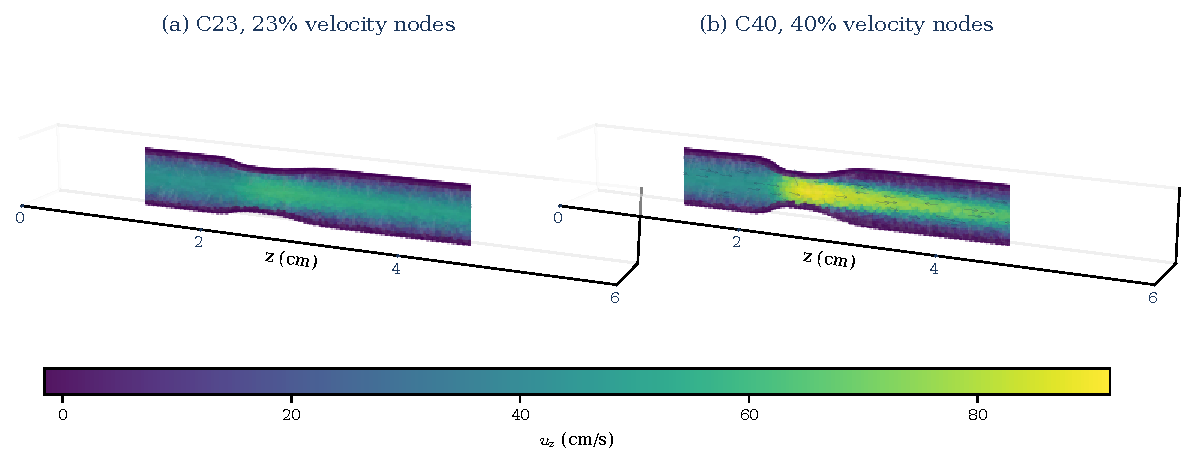
\includegraphics[width=\textwidth]{report/assets/rendered/resolved-3d-flow-field.pdf}
    }{%
        \fbox{\parbox{0.82\linewidth}{\centering Resolved velocity-field
        asset unavailable in this checkout.}}
    }
    \caption{Final-time resolved velocity samples used by the 23\% and 40\%
    stenosis comparisons. The panels show node-centered $u_z$ values; the
    quantitative comparison enters only after applying the declared
    cross-sectional observation operator.}
    \label{fig:resolved-3d-flow-field}
\end{figure}

\begin{table}[!htb]
    \centering
    \scriptsize
    \caption{Subcritical-boundary diagnostics for the same two 1D runs used in
    the resolved-velocity comparison. The characteristic-radicand values are in
    solver units of cm$^2$/s$^2$; the signs of $\lambda_-$ and $\lambda_+$
    support the boundary-regime gate in
    Assumption~\ref{ass:1d-subcritical-boundary-regime}.}
    \label{tab:t1-alpha-radicand-diagnostics}
    \resizebox{\textwidth}{!}{%
    \begin{tabular}{@{}lrrrrrrrr@{}}
        \toprule
        \textbf{Case}
            & $\boldsymbol{\min \alpha_{\mathrm{eff}}}$
            & $\boldsymbol{\max \alpha_{\mathrm{eff}}}$
            & $\boldsymbol{\min \chi^2}$
            & $\boldsymbol{\min\lambda_-}$
            & $\boldsymbol{\max\lambda_-}$
            & $\boldsymbol{\min\lambda_+}$
            & $\boldsymbol{\max\lambda_+}$
            & $\boldsymbol{\min\{\lambda_+,-\lambda_-\}}$ \\
        \midrule
        23\% stenosis & 1.33058 & 1.33333 & $8.15\times 10^5$ & -998.85 & -852.17 & 953.33 & 1058.76 & 852.17 \\
        40\% stenosis & 1.32500 & 1.33333 & $6.36\times 10^5$ & -999.08 & -713.79 & 880.69 & 1058.94 & 713.79 \\
        \bottomrule
    \end{tabular}
    }
\end{table}

\begin{table}[!htb]
    \centering
    \scriptsize
    \pgfplotstableread[col sep=space]{report/assets/data/stenosis-comparison/production-diagnostics-reference.dat}\TOneProductionDiagnostics
    \caption{Production diagnostics from the 23\% and 40\% severity 1D
    comparison runs completed at $T=0.9995$ s. These rows summarize timestep,
    CFL, positivity, area, and finite-volume bookkeeping for the 1D runs used
    in the resolved-comparator evidence.}
    \label{tab:t1-production-diagnostics}
    \resizebox{\textwidth}{!}{%
    \pgfplotstabletypeset[
        columns={
            case,
            target_time,
            completed_time,
            cross_model_time_offset,
            dt_min,
            dt_max,
            cfl_max,
            min_Aphys,
            volume_defect,
            positivity_count,
            area_flux_balance,
            rhs_area_max,
            rhs_flow_max
        },
        every head row/.style={before row=\toprule, after row=\midrule},
        every last row/.style={after row=\bottomrule},
        columns/case/.style={string type,column type=l,column name=\textbf{Stenosis}},
        columns/target_time/.style={fixed,precision=4,column name=$\boldsymbol{T_{\mathrm{target}}}$},
        columns/completed_time/.style={fixed,precision=4,column name=$\boldsymbol{T_{\mathrm{done}}}$},
        columns/cross_model_time_offset/.style={sci,precision=2,column name=$\boldsymbol{|\Delta t_{\mathrm{1D--3D}}|}$},
        columns/dt_min/.style={sci,precision=2,column name=$\boldsymbol{\Delta t_{\min}}$},
        columns/dt_max/.style={sci,precision=2,column name=$\boldsymbol{\Delta t_{\max}}$},
        columns/cfl_max/.style={fixed,precision=2,column name=\textbf{CFL$_{\max}$}},
        columns/min_Aphys/.style={fixed,precision=5,column name=$\boldsymbol{\min \pi a}$},
        columns/volume_defect/.style={sci,precision=2,column name=$\boldsymbol{\Delta\!\int a\,dz}$},
        columns/positivity_count/.style={int detect,column name=\textbf{pos. count}},
        columns/area_flux_balance/.style={sci,precision=2,column name=\textbf{area-flux balance}},
        columns/rhs_area_max/.style={sci,precision=2,column name=$\boldsymbol{\max|\dot a|}$},
        columns/rhs_flow_max/.style={fixed,precision=5,column name=$\boldsymbol{\max|\dot q|}$}
    ]\TOneProductionDiagnostics
    }
\end{table}

\FloatBarrier

\subsubsection{Observation Operator and Deformed Coordinates}
\label{subsec:cross-sectional-sampling-protocol-results}

The comparison uses the declared \texttt{CrossSectionQuadratureOperator}. For a
target plane $S_j=\Omega_{\mathrm{3D}}\cap\{z=z_j\}$, the operator intersects
the tetrahedral mesh with the plane, triangulates the cut polygon, and computes
\begin{flalign*}
    \quad
    A_{3D,j}
    =
    \sum_{\Delta\in\mathcal Q_j}|\Delta|,
    \qquad
    Q_{3D,j}
    =
    \sum_{\Delta\in\mathcal Q_j}|\Delta|\,\bar u_{z,\Delta},
    \qquad
    \bar u_{3D,j}
    =
    Q_{3D,j}/A_{3D,j}. &&
\end{flalign*}
The 1D quantities use the solver-to-physical map
$Q_{1D,j}=\pi q(z_j,t)$ and $\bar u_{1D,j}=q(z_j,t)/a(z_j,t)$. In
deformed-coordinate mode the plane cut is formed after replacing each mesh
coordinate $x$ by $x+d(x)$, where $d$ is the node-centered resolved
displacement field.

The stenosis throat is the minimizer $z^\star=\argmin_z R_0(z)$ of the smooth
reference-radius profile in Eq.~\ref{eq:1d-stenosis-profile}. For the comparison
geometry this gives $z^\star\approx2.451\,\mathrm{cm}$, with
$R_{\min}=0.1386\,\mathrm{cm}$ for the 23\% stenosis case and
$R_{\min}=0.1080\,\mathrm{cm}$ for the 40\% stenosis case.

\begin{table}[!htb]
    \centering
    \scriptsize
    \caption{Cut-area check against the static reference
    $A_{\mathrm{ref}}(z)=\pi R_0(z)^2$ for both coordinate choices.
    Discrepancies are percentages over the 200 valid section targets.}
    \label{tab:t1-area-check}
    \begin{tabular}{@{}llrrrr@{}}
        \toprule
        \textbf{Case}
            & \textbf{Coordinates}
            & $\boldsymbol{\min \epsilon_A}$
            & $\boldsymbol{\mathrm{median}\ \epsilon_A}$
            & $\boldsymbol{\mathrm{mean}\ \epsilon_A}$
            & $\boldsymbol{\max \epsilon_A}$ \\
        \midrule
        23\% stenosis & reference & 0.045 & 0.281 & 0.389 & 2.94 \\
        23\% stenosis & deformed & 0.001 & 0.254 & 0.336 & 3.03 \\
        40\% stenosis & reference & 0.005 & 0.291 & 0.397 & 4.46 \\
        40\% stenosis & deformed & 0.003 & 0.286 & 0.417 & 4.60 \\
        \bottomrule
    \end{tabular}
\end{table}

\subsubsection{Reference-Coordinate Velocity Comparison}
\label{subsec:section-mean-velocity-discrepancies}

The reference-coordinate comparison is retained as the baseline final-time
velocity comparison. The section means are
$\langle Q_{1D}\rangle=2.288\,\mathrm{cm}^3/\mathrm{s}$ and
$\langle Q_{3D}\rangle=2.241\,\mathrm{cm}^3/\mathrm{s}$ for the 23\% stenosis
case, and $\langle Q_{1D}\rangle=2.287\,\mathrm{cm}^3/\mathrm{s}$ and
$\langle Q_{3D}\rangle=2.219\,\mathrm{cm}^3/\mathrm{s}$ for the 40\% stenosis
case.

\begin{figure}[!htb]
    \centering
    \captionsetup{aboveskip=2pt,belowskip=2pt}
    \figtikz{axial-flow-comparison}
    \caption{Axial physical-flow comparison after applying the
    reference-coordinate plane-quadrature observation operator. Dashed curves
    are $Q_{1D}(z)=\pi q(z)$ and solid curves are $Q_{3D}(z)$ from the resolved
    velocity fields; the figure compares observed section flow, not native
    resolved velocity fields or pressure-ratio output.}
    \label{fig:t1-axial-flow-comparison}
\end{figure}

The algebraic split used for flow/area bookkeeping is
\begin{flalign*}
    \quad
    \frac{Q_{1D}}{A_{1D}}-\frac{Q_{3D}}{A_{3D}}
    =
    \frac{Q_{1D}-Q_{3D}}{A_{1D}}
    +
    Q_{3D}\left(\frac{1}{A_{1D}}-\frac{1}{A_{3D}}\right),
    \qquad A_{1D}=\pi a. &&
\end{flalign*}
This decomposition is bookkeeping for the sampled sections, not causal
attribution.

\begin{table}[!htb]
    \centering
    \scriptsize
    \caption{Section-wise decomposition of the reference-coordinate
    mean-velocity discrepancy into physical-flow and area-denominator
    contributions. Values are in cm/s. This bookkeeping split is tied to the
    declared section observation operator and is not a causal error
    attribution.}
    \label{tab:t1-flow-area-decomposition}
    \resizebox{\textwidth}{!}{%
    \begin{tabular}{@{}lrrrrl@{}}
        \toprule
        \textbf{Case}
            & $\boldsymbol{\langle |(Q_{1D}-Q_{3D})/A_{1D}|\rangle}$
            & $\boldsymbol{\langle |Q_{3D}(A_{1D}^{-1}-A_{3D}^{-1})|\rangle}$
            & $\boldsymbol{z_{\max |d_u|}}$
            & $\boldsymbol{|d_u|_{\max}}$
            & \textbf{Larger bookkeeping term at max} \\
        \midrule
        23\% stenosis & 0.529 & 0.112 & 2.291 & 2.35 & Flow term \\
        40\% stenosis & 1.012 & 0.133 & 2.261 & 9.92 & Flow term \\
        \bottomrule
    \end{tabular}%
    }
\end{table}

\begin{table}[!htb]
    \centering
    \scriptsize
    \caption{Reference-coordinate section-mean velocity discrepancy summary at
    the matched final-time sample after applying the common section observation
    map. Values are in cm/s except for the axial location column in cm; the
    table reports diagnostic cross-model discrepancy, not clinical validation.}
    \label{tab:t1-3d-comparison-summary}
    \resizebox{\textwidth}{!}{%
    \begin{tabular}{@{}lrrrrrrrrr@{}}
        \toprule
        \textbf{Case}
            & \textbf{Sections}
            & $\boldsymbol{\langle\bar u_{1D}\rangle}$
            & $\boldsymbol{\langle\bar u_{3D}\rangle}$
            & $\boldsymbol{\overline d_u}$
            & $\boldsymbol{D_{u,1}}$
            & $\boldsymbol{D_{u,2}}$
            & \textbf{rel.} $\boldsymbol{D_{u,2}}$
            & $\boldsymbol{\max |d_u|}$
            & $\boldsymbol{z_{\max |d_u|}}$ \\
        \midrule
        23\% stenosis & 200 & 24.11 & 23.63 & 0.480 & 0.505 & 0.664 & 0.0277 & 2.35 & 2.291 \\
        40\% stenosis & 200 & 26.43 & 25.52 & 0.909 & 0.966 & 1.87 & 0.0688 & 9.92 & 2.261 \\
        \bottomrule
    \end{tabular}
    }
\end{table}

\begin{figure}[!htb]
    \centering
    \captionsetup{aboveskip=2pt,belowskip=2pt}
    \figtikz{section-mean-comparison}
    \caption{Area-mean axial velocity comparison at $t=0.9995$ s under the
    reference-coordinate section observation map. Solid curves are tetrahedral
    cross-section quadrature means from the resolved 3D velocity field; dashed
    curves are interpolated 1D means
    $\bar u=q/a=Q_{\mathrm{phys}}/A_{\mathrm{phys}}$.}
    \label{fig:t1-section-mean-comparison}
\end{figure}

\begin{table}[!htb]
    \centering
    \scriptsize
    \caption{Normalized scale comparison between the production-grid
    geometry-rest limitation and final-time 1D--3D velocity-discrepancy
    measures. These ratios place the diagnostic comparison on a common scale;
    they do not convert the comparison into an accepted-reference validation
    result.}
    \label{tab:t1-normalized-scale-comparison}
    \begin{tabular}{@{}lrrrr@{}}
        \toprule
        \textbf{Case}
            & \textbf{rest }$\boldsymbol{\max |q|}$\textbf{/prod. }$\boldsymbol{q}$
            & $\boldsymbol{D_{Q,1}/\langle Q_{1D}\rangle}$
            & $\boldsymbol{D_{u,1}}$ \textbf{(cm/s)}
            & \textbf{rel. }$\boldsymbol{D_{u,2}}$ \\
        \midrule
        23\% stenosis & 5.27\% & 2.11\% & 0.505 & 2.77\% \\
        40\% stenosis & 8.71\% & 3.10\% & 0.966 & 6.88\% \\
        \bottomrule
    \end{tabular}
\end{table}

\begin{table}[!htb]
    \centering
    \scriptsize
    \caption{Optional production-grid sensitivity for the reference-coordinate
    resolved-velocity observation map. Flow discrepancies are in cm$^3$/s and
    velocity discrepancies are in cm/s; the rows test numerical sensitivity of
    the comparison output, not patient-specific interpretation.}
    \label{tab:t1-grid-sensitivity-summary}
    \resizebox{\textwidth}{!}{%
    \begin{tabular}{llrrrrrrr}
\toprule
Case & $N$ & $D_{Q,1}$ & $D_{Q,2}$ & $D_{u,1}$ & $D_{u,2}$ & rel. $D_{u,2}$ & max $|d_u|$ & adj. $D_{u,2}$ \\
\midrule
23\% stenosis & 200 & 0.05965 & 0.07358 & 0.6182 & 0.8996 & 0.03757 & 4.533 & -- \\
23\% stenosis & 400 & 0.04821 & 0.05085 & 0.5048 & 0.6636 & 0.02771 & 2.349 & 0.678 \\
23\% stenosis & 800 & 0.04874 & 0.05322 & 0.5049 & 0.7063 & 0.0295 & 2.94 & 0.1785 \\
40\% stenosis & 200 & 0.08395 & 0.1132 & 1.082 & 1.894 & 0.06975 & 7.93 & -- \\
40\% stenosis & 400 & 0.07087 & 0.08927 & 0.966 & 1.868 & 0.06881 & 9.923 & 1.328 \\
40\% stenosis & 800 & 0.07108 & 0.09539 & 0.9843 & 2.019 & 0.07435 & 11.57 & 0.3499 \\
\bottomrule
\end{tabular}
%
    }
\end{table}

\begin{table}[!htb]
    \centering
    \scriptsize
    \caption{Five largest section-wise velocity discrepancies in the
    reference-coordinate comparison. Velocities and velocity discrepancies are
    in cm/s; physical flows and flow discrepancies are in cm$^3$/s. The ranking
    identifies where the declared observation map differs most strongly between
    tiers.}
    \label{tab:t1-largest-section-discrepancies}
    \begin{tabular}{@{}rlrrrrrrrr@{}}
        \toprule
        \textbf{Rank}
            & \textbf{Case}
            & $\boldsymbol{z}$ \textbf{(cm)}
            & $\boldsymbol{\bar u_{1D}}$
            & $\boldsymbol{\bar u_{3D}}$
            & $\boldsymbol{|d_u|}$
            & $\boldsymbol{Q_{1D}}$
            & $\boldsymbol{Q_{3D}}$
            & $\boldsymbol{|d_Q|}$
            & \textbf{Tri.} \\
        \midrule
        1 & 40\% stenosis & 2.261 & 52.58 & 42.66 & 9.92 & 2.201 & 1.862 & 0.339 & 759 \\
        2 & 40\% stenosis & 2.291 & 56.94 & 48.20 & 8.74 & 2.230 & 1.903 & 0.327 & 749 \\
        3 & 40\% stenosis & 2.352 & 61.43 & 53.22 & 8.21 & 2.270 & 1.980 & 0.290 & 743 \\
        4 & 40\% stenosis & 2.322 & 59.81 & 52.09 & 7.72 & 2.253 & 1.970 & 0.283 & 771 \\
        5 & 40\% stenosis & 2.231 & 46.95 & 39.94 & 7.01 & 2.174 & 1.918 & 0.256 & 833 \\
        \bottomrule
    \end{tabular}
\end{table}

\subsubsection{Deformed-Coordinate Comparison}
\label{subsec:deformed-coordinate-comparison}

The deformed-coordinate comparison repeats the same section operator after
moving each resolved node by its displacement value. Table~\ref{tab:t1-coordinate-mode-comparison}
shows that applying displacement changes the final-time discrepancy measures
only modestly for these two datasets. This is still not a full wall-motion
match: the available comparison record contains the final displacement field, not the
resolved wall history or boundary histories.

\begin{table}[!htb]
    \centering
    \scriptsize
    \caption{Reference-coordinate versus deformed-coordinate discrepancy
    measures for the same section observation map. $D_{u,1}$ and $D_{u,2}$ are
    the mean absolute and RMS section-mean velocity discrepancies in cm/s;
    $D_{Q,1}$ is the mean absolute physical-flow discrepancy in cm$^3$/s.}
    \label{tab:t1-coordinate-mode-comparison}
    \begin{tabular}{@{}llrrrr@{}}
\toprule
Case & Coordinates & $D_{u,1}$ & $D_{u,2}$ & $\max |d_u|$ & $D_{Q,1}$ \\
\midrule
C23 (22.56\%) & reference & 0.6040 & 1.070 & 11.400 & 0.06259 \\
C23 (22.56\%) & deformed & 0.6111 & 1.073 & 11.400 & 0.06184 \\
40\% stenosis & reference & 1.1318 & 2.292 & 12.291 & 0.08514 \\
40\% stenosis & deformed & 1.1410 & 2.294 & 12.304 & 0.08420 \\
\bottomrule
\end{tabular}

\end{table}

\begin{figure}[!htb]
    \centering
    \captionsetup{aboveskip=2pt,belowskip=2pt}
    \figtikz{coordinate-mode-discrepancy}
    \caption{Effect of the displacement-aware observation map on the
    section-wise velocity discrepancy. Solid curves use reference mesh
    coordinates, while dashed curves form the same plane cuts after the nodal
    map $x\mapsto x+d(x)$; the figure changes the coordinate mode, not the 1D
    model or the resolved velocity field.}
    \label{fig:t1-coordinate-mode-discrepancy}
\end{figure}

\subsubsection{Quasi-static Membrane-FSI Comparator}
\label{subsec:membrane-fsi-comparator}

The resolved wall comparator solves a quasi-static fixed point between the
Stokes lumen solve and the radial membrane update. In the notation of
Appendix~\ref{app:num-membrane-fsi-validation}, the wall equation is the
inertia-free form
\begin{flalign*}
    \quad
    C_0\eta_r(z)=f_r(z),
    \qquad
    \eta_r(0)=\eta_r(L)=0,
    \qquad
    C_0=\frac{Eh}{(1-\sigma^2)(R_0^*)^2}. &&
\end{flalign*}
This is the Canic-style membrane relation used for the resolved comparator
\cite[Eq.~(35)]{CanicEtAl2024Extended1DStenosis}. It is separate from the
selected 1D pressure--area closure used in the reduced model. The retained
comparator is a quasi-static radial membrane update coupled to repeated Stokes
solves; it informs wall-motion scale, not full transient moving-boundary FSI
validation.

\begin{table}[!htb]
    \centering
    \scriptsize
    \caption{Quasi-static membrane-FSI fixed-point results on the retained
    finer mesh. The reported displacement is the radial wall displacement
    $\eta_r$; the minimum radius is the deformed lumen radius
    $R_0+\eta_r$. This comparator informs wall-motion scale only and does not
    supply a transient FSI validation target.}
    \label{tab:t1-membrane-fsi-summary}
    \begin{tabular}{@{}lrrrrrr@{}}
\toprule
Case & Mesh & Iter. & Residual (cm) & $\max\eta$ (cm) & $\min R$ (cm) & $\langle Q\rangle$ (cm$^3$/s) \\
\midrule
C23 (22.56\%) & $16\times4\times16$ & 9 & 5.972e-8 & 3.052e-5 & 0.1402 & 0.5472 \\
40\% stenosis & $16\times4\times16$ & 9 & 6.051e-8 & 3.092e-5 & 0.1108 & 0.416 \\
\bottomrule
\end{tabular}

\end{table}

\begin{figure}[!htb]
    \centering
    \captionsetup{aboveskip=2pt,belowskip=2pt}
    \resizebox{0.98\textwidth}{!}{\figtikz{membrane-fsi-wall-profile}}
    \caption{Quasi-static wall deformation from the membrane-FSI comparator.
    The upper panel shows the radial displacement $\eta_r(z)$ solving the
    fixed-end membrane equation; the lower panel shows the resulting deformed
    radius $R_0(z)+\eta_r(z)$ alongside the reference radius.}
    \label{fig:t1-membrane-fsi-wall-profile}
\end{figure}

\begin{figure}[!htb]
    \centering
    \captionsetup{aboveskip=2pt,belowskip=2pt}
    \resizebox{0.98\textwidth}{!}{\figtikz{membrane-fsi-fixed-point-history}}
    \caption{Fixed-point convergence for the quasi-static membrane-FSI
    comparator. The residual is the maximum radial-radius update between
    successive coupled wall solves, reported in centimeters; it checks the
    comparator solve, not the 1D--3D velocity observation error.}
    \label{fig:t1-membrane-fsi-fixed-point-history}
\end{figure}

\subsubsection{Radial-Profile Audit}
\label{subsec:reconstructed-radial-profile-results}

The radial-profile reducer was rerun for slices
$z=1.951$, $2.451$, and $2.951\,\mathrm{cm}$ in both reference and deformed
coordinate modes. Its summary-discrepancy recomputation matched the generated
radial summaries, but the area-closure gate failed because those slices are not
members of the retained 200-section axial target set. The radial-profile plot is
therefore not promoted into the main evidence.

\begin{table}[!htb]
    \centering
    \scriptsize
    \caption{Radial-profile promotion check. The zero summary delta confirms
    that the raw radial rows reproduce the generated radial-summary statistic;
    the area-closure gate remains failed, so no radial figure or radial-bin
    localization claim is retained.}
    \label{tab:t1-radial-profile-audit}
    \begin{tabular}{@{}llrrrl@{}}
\toprule
Case & Coordinates & Slices & Bins & Summary delta & Audit result \\
\midrule
C23 (22.56\%) & reference & 3 & 20 & 0.0 & not_evaluated: matching section row unavailable at radial z-slice; section area unavailable; section flow unavailable \\
C23 (22.56\%) & deformed & 3 & 20 & 0.0 & not_evaluated: matching section row unavailable at radial z-slice; section area unavailable; section flow unavailable \\
40\% stenosis & reference & 3 & 20 & 0.0 & not_evaluated: matching section row unavailable at radial z-slice; section area unavailable; section flow unavailable \\
40\% stenosis & deformed & 3 & 20 & 0.0 & not_evaluated: matching section row unavailable at radial z-slice; section area unavailable; section flow unavailable \\
\bottomrule
\end{tabular}

\end{table}

\subsubsection{Interpretation Limits}
\label{subsec:spatial-localization-discrepancies}

This chapter reports a controlled diagnostic cross-model comparison against
declared resolved comparators: a reference-coordinate velocity comparison, a
displacement-aware observation comparison, and a quasi-static membrane-wall
comparator. The evidence supports the implemented observation and comparison
workflow and localizes final-time velocity discrepancies under the stated
operators. It does not provide externally validated clinical prediction
evidence, pressure-ratio evidence, or equivalence to a full transient FSI
computation with matched boundary and wall-history data.


\FloatBarrier
